\documentclass[tikz,border=10pt]{standalone}
\usetikzlibrary{arrows.meta, positioning, calc}
\usepackage{amsmath}
\usepackage{amssymb}

\begin{document}
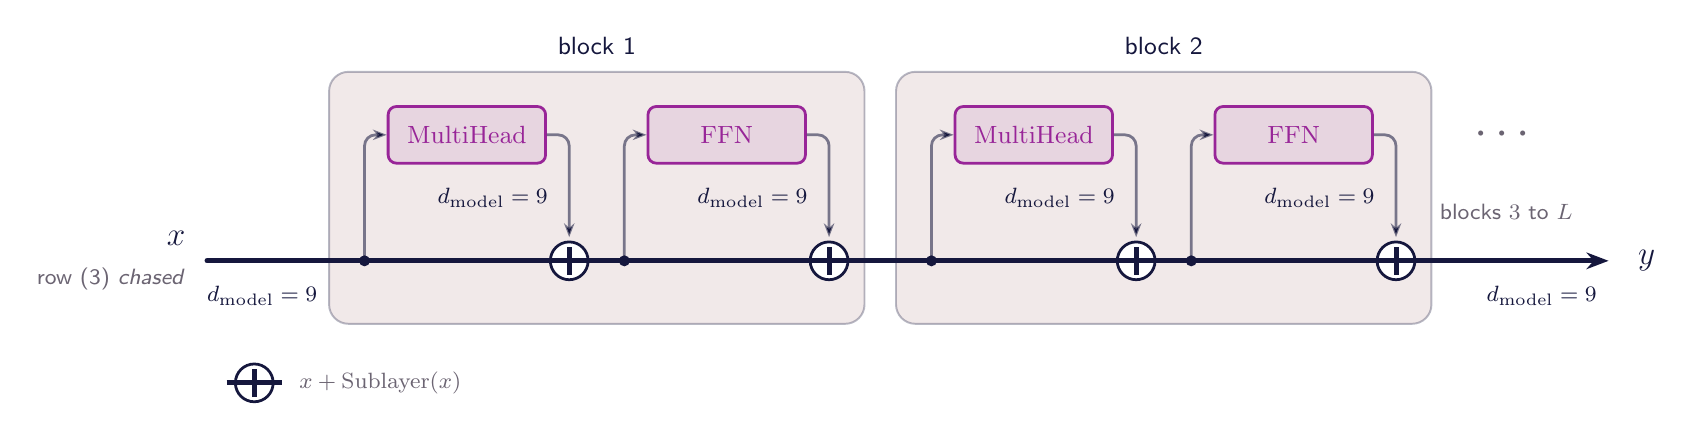
\begin{tikzpicture}[
    every node/.style={font=\sffamily},
]

\definecolor{c1}{HTML}{15173D}
\definecolor{c2}{HTML}{982598}
\definecolor{c3}{HTML}{E491C9}
\definecolor{c4}{HTML}{F1E9E9}
\definecolor{axiscolor}{HTML}{333333}
\definecolor{labelcolor}{HTML}{6B6472}

% ================================================================
%  GEOMETRY, planned before any TikZ was written.
%
%  The stream runs horizontally along y = 0, left to right, c1 at
%  1.8pt, unbroken from x = -0.6 to the arrowhead at x = 17.2.
%  Nothing sits ON it: every sublayer hangs above it.
%
%  ONE SUBLAYER UNIT, tap at x = T (matches prenorm_postnorm pitch):
%     riser up at T          to y = 1.6
%     box centred (T + 1.3, 1.6), 2.0 x 0.72
%     riser down at T + 2.6  into the add at (T + 2.6, 0)
%  Both sublayers ABOVE the stream, as in prenorm_postnorm and
%  transformer_block; no alternation.  Two blocks plus a continuation
%  keeps the figure ~19cm wide so \footnotesize survives 768px.
%
%  Block b at bx:  MultiHead tap bx,     add bx+2.6
%                  FFN       tap bx+3.3, add bx+5.9
%     bx = 1.4 (panel 0.95..7.75) and bx = 8.6 (panel 8.15..14.95)
%     panels y in [-0.8, 2.4], titles at y = 2.5
%  continuation: dots at (15.9, 1.6), label under at (15.9, 0.62)
%
%  THE ADD, identical everywhere (drawn by \addsym):
%     stream (already down) -> white disc r = 0.24, c1 stroke 1.0pt
%     -> re-stroke the stream across the disc, c1 at 1.8pt
%     -> vertical stroke, c1 at 1.8pt, half-length 0.18
%  Nothing else inside the disc.  Taps are small c1 dots (r = 0.07)
%  sitting 0.7 clear of any disc.
%
%  Width stamps, c1: below the stream at x = 0.35 and x = 16.3, and
%  one per branch return at (add - 0.15, 0.80), anchored east so the
%  text runs back under its own box and never near the next riser.
%  Key for the add symbol: (0.0, -1.55), drawn by the same macro.
% ================================================================

\tikzset{
  stream/.style={draw=c1, line width=1.8pt, line cap=round},
  sub/.style={draw=c2, line width=1.0pt, fill=c2, fill opacity=0.10,
              text opacity=1, text=c2, rounded corners=3pt,
              minimum width=2.0cm, minimum height=0.72cm, inner sep=1pt,
              font=\sffamily\small},
  br/.style={-{Stealth[length=5pt]}, line width=1.0pt, draw=c1,
             draw opacity=0.55, rounded corners=4pt},
  panel/.style={fill=c4, rounded corners=7pt, draw=c1, draw opacity=0.30,
                line width=0.7pt},
  wid/.style={font=\sffamily\footnotesize, text=c1},
  title/.style={font=\sffamily\small, text=c1, anchor=south},
  key/.style={font=\sffamily\footnotesize, text=labelcolor},
}

% the residual add: the stream itself is the horizontal bar of the plus
\newcommand{\addsym}[2]{%
  \fill[white] (#1, #2) circle (0.24);
  \draw[draw=c1, line width=1.0pt] (#1, #2) circle (0.24);
  \draw[draw=c1, line width=1.8pt] ({#1-0.26}, #2) -- ({#1+0.26}, #2);
  \draw[draw=c1, line width=1.8pt] (#1, {#2-0.18}) -- (#1, {#2+0.18});
}

% ---------------------------------------------------------------- panels
\foreach \bx/\b in {1.4/1, 8.6/2} {
    \draw[panel] ({\bx-0.45}, -0.8) rectangle ({\bx+6.35}, 2.4);
    \node[title] at ({\bx+2.95}, 2.5) {block \b};
}

% ---------------------------------------------------------------- the stream
\draw[stream, -{Stealth[length=8pt]}] (-0.6, 0) -- (17.2, 0);

% ---------------------------------------------------------------- sublayers
\foreach \bx/\b in {1.4/1, 8.6/2} {
    \foreach \t/\nm/\s in {0/MultiHead/m, 3.3/FFN/f} {
        \pgfmathsetmacro{\T}{\bx + \t}
        \pgfmathsetmacro{\A}{\T + 2.6}
        \node[sub] (\s\b) at ({\T + 1.3}, 1.6) {$\mathrm{\nm}$};
        \draw[br] (\T, 0) -- (\T, 1.6) -- (\s\b.west);
        \draw[br] (\s\b.east) -- (\A, 1.6) -- (\A, 0.30);
        \fill[c1] (\T, 0) circle (0.07);
        \node[wid, anchor=east] at ({\A - 0.15}, 0.80)
            {$d_{\mathrm{model}} = 9$};
    }
}

% ---------------------------------------------------------------- adds
\foreach \bx in {1.4, 8.6} {
    \foreach \d in {2.6, 5.9} { \addsym{\bx+\d}{0} }
}

% ---------------------------------------------------------------- continuation
\node[font=\sffamily\LARGE, text=labelcolor] at (15.9, 1.6) {$\cdots$};
\node[font=\sffamily\footnotesize, text=labelcolor] at (15.9, 0.62)
    {blocks $3$ to $L$};

% ---------------------------------------------------------------- ends
\node[anchor=east, align=right] at (-0.75, 0)
    {{\large\textcolor{c1}{$x$}}\\[2pt]
     {\footnotesize\textcolor{labelcolor}{row (3) \emph{chased}}}};
\node[anchor=west] at (17.45, 0) {{\large\textcolor{c1}{$y$}}};

\node[wid, anchor=north] at (0.1, -0.20) {$d_{\mathrm{model}} = 9$};
\node[wid, anchor=north] at (16.35, -0.20) {$d_{\mathrm{model}} = 9$};

% ---------------------------------------------------------------- key
\draw[draw=c1, line width=1.8pt] (-0.35, -1.55) -- (0.35, -1.55);
\addsym{0.0}{-1.55}
\node[key, anchor=west] at (0.45, -1.55) {$x + \mathrm{Sublayer}(x)$};

\end{tikzpicture}
\end{document}
